\documentclass[10pt]{book}
\usepackage{commands}

\usepackage{bbm}

\newcommand{\Aut}{\operatorname{Aut}}
\newcommand{\SLNR}{\operatorname{SL}(n,\R)}
\newcommand{\GLNR}{\operatorname{GL}(n,\R)}

\begin{document}




\begin{tikzpicture}[remember picture,overlay]
	% If a chapter image has been specified
	\expandafter\ifstrequal\expandafter{\thechapterimage}{}{}{
		% Output the chapter image
		\node[
		anchor=north west, % Anchor point on the image
		inner sep=0pt, % Inner padding
		] at (current page.north west) {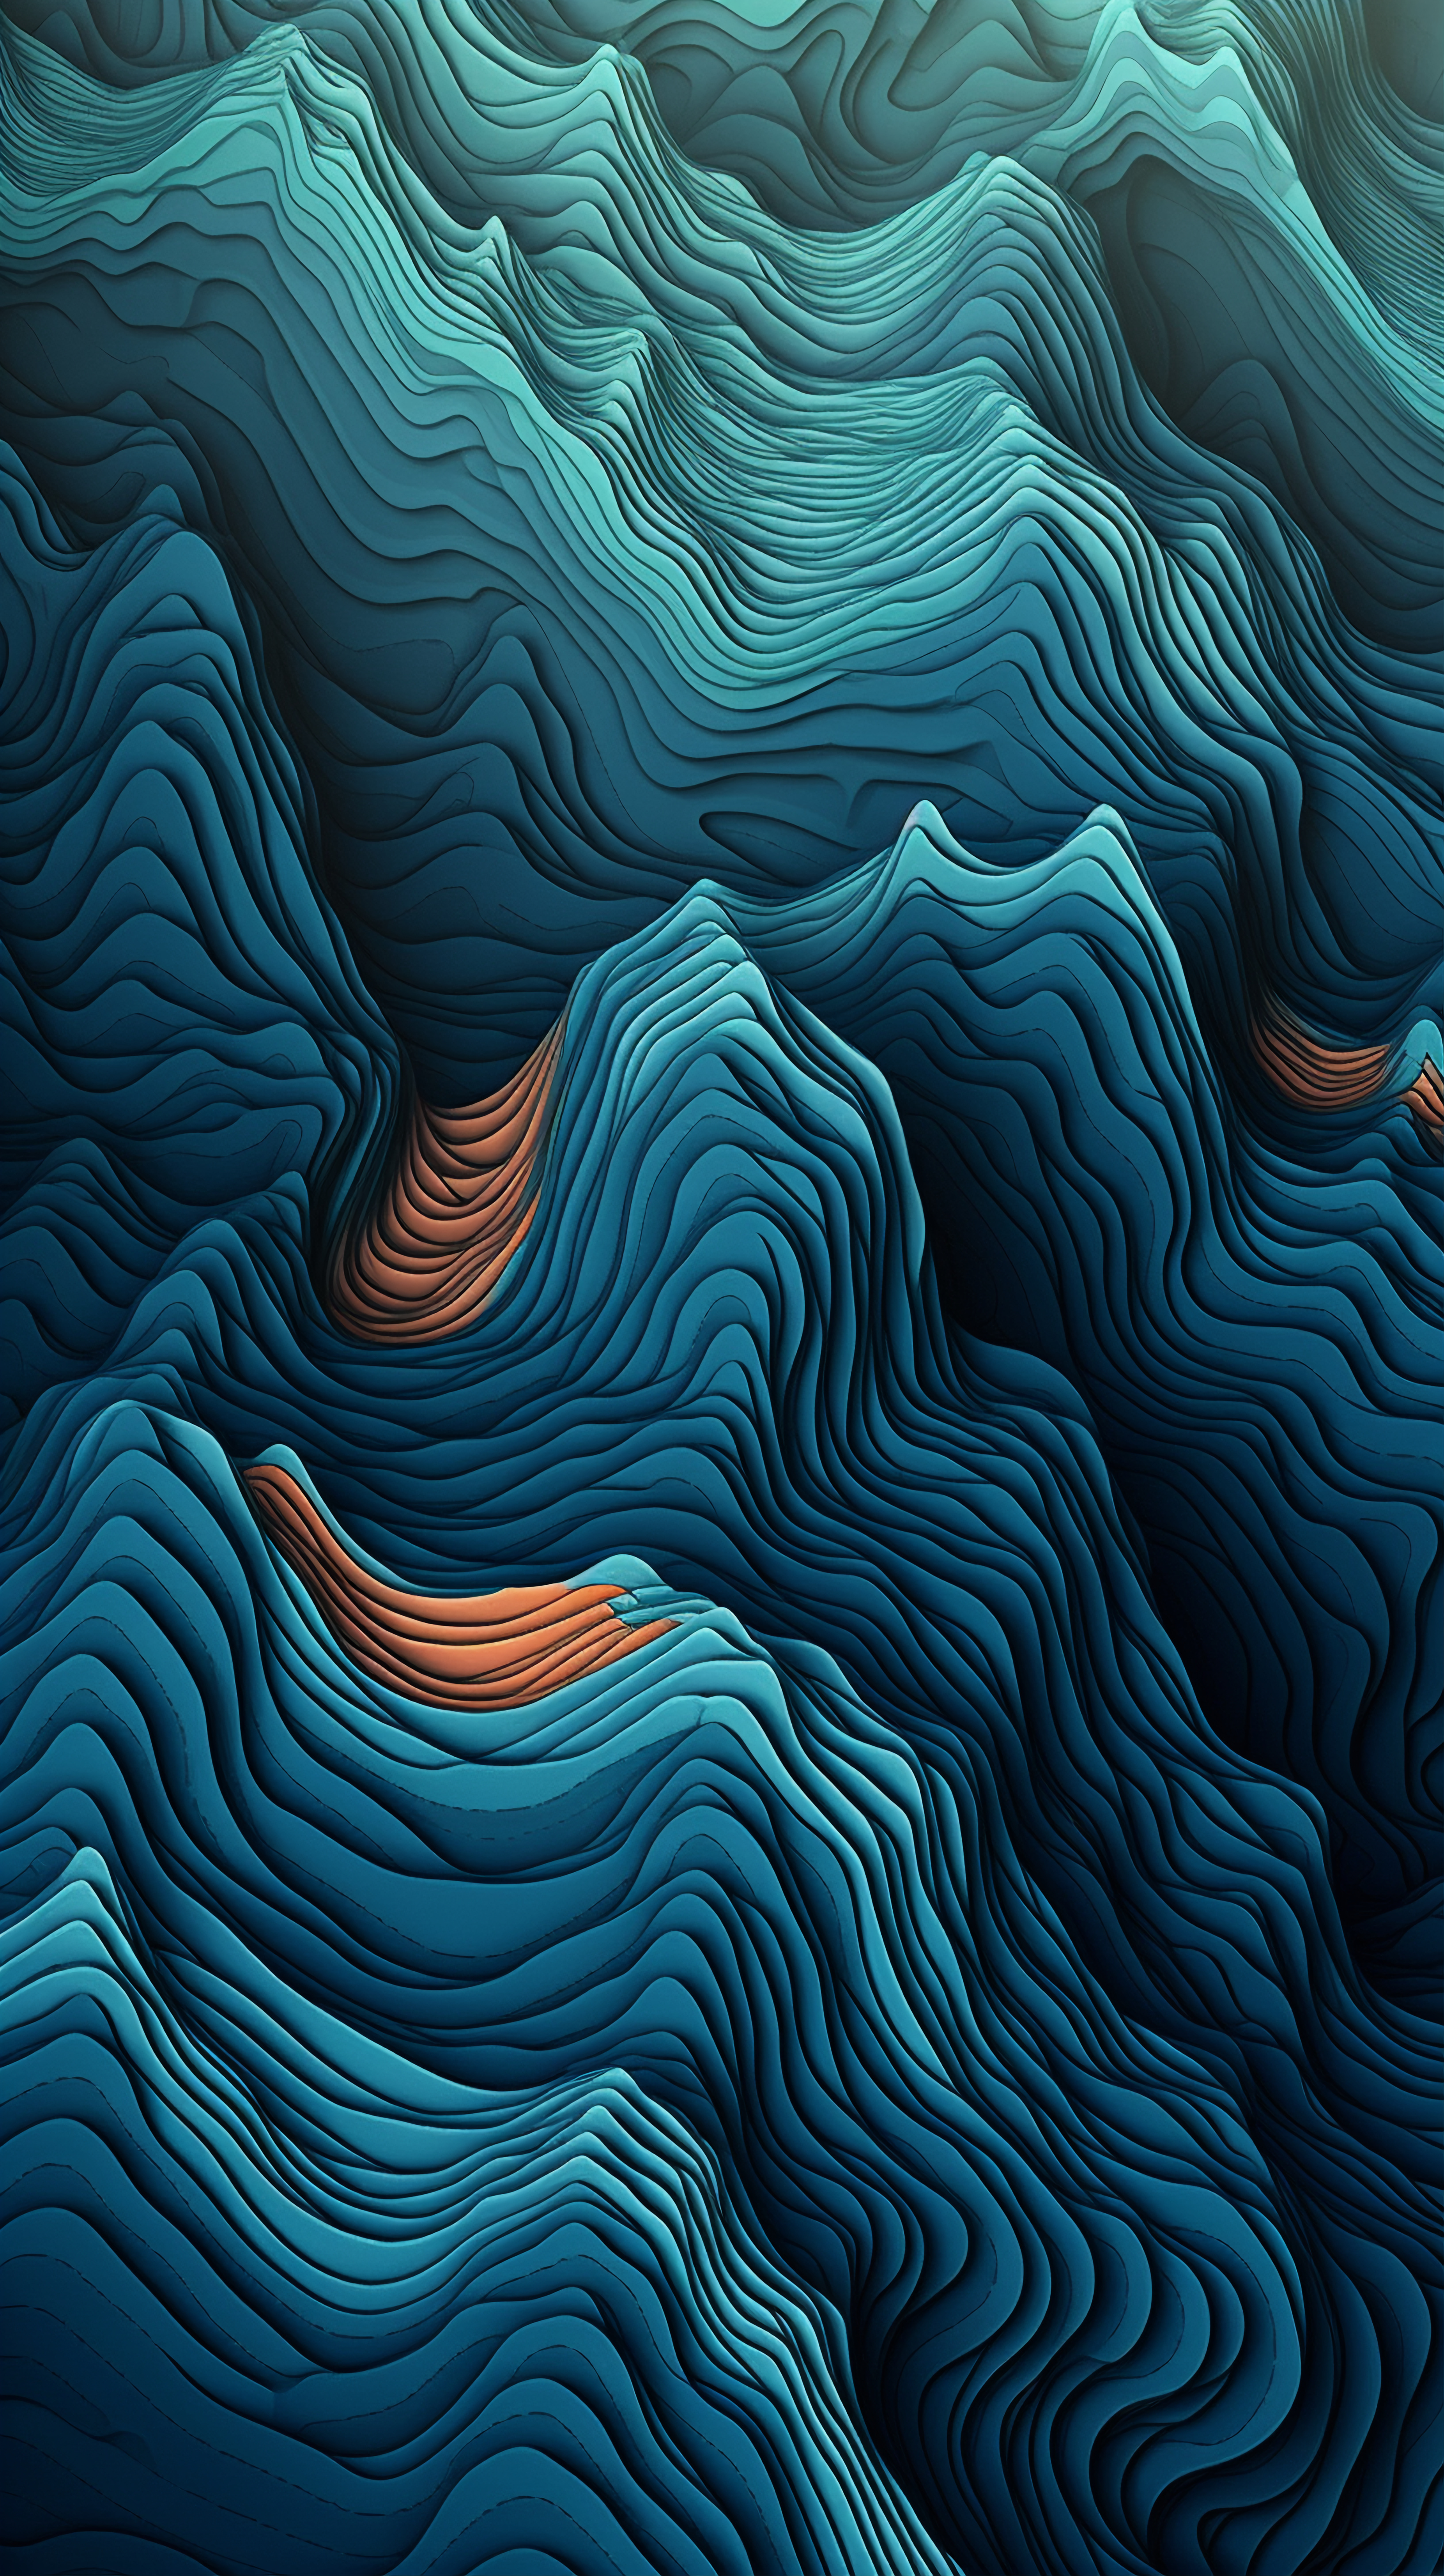
\includegraphics[angle=0,width=\paperwidth]{Images/output}};
	}
\end{tikzpicture}

\vspace{7cm}

\heading{Linear Operator Theory}


%\begin{figure}[h!]
%	\centering
%	\includegraphics[width=1\linewidth]{Images/realAnalysis}
%	\caption*{$\mathbb{R}$eal Analysis, Created by DALL-E!}
%	\label{fig:realanalysis}
%	
%\end{figure}




\tableofcontents


\chapter{Topological Spaces}


\section{Solved Problems}


\begin{problem}
	Let $ d $ be a metric on $ X $ and let $ d_\alpha = \alpha d $, where $ 0 < \alpha < 1 $. Show that $ d_\alpha \not\equiv d $ if $ X $ has more than two points.
\end{problem}
\begin{solution}
	Let $ X $ have more than one point. Then $ \exists x,y \in X $ such that $ d(x,y) \neq 0 $. Then $ d(x,y) \neq \alpha d(x,y) = d_\alpha(x,y) $. So $ d \not\equiv d_\alpha $.
\end{solution}


\begin{problem}
	Show that $ d(x,y) = \abs{x-y} $ is a metric on the real number $ \R $. Show that it is also a metric on the set of complex numbers $ \C $.
\end{problem}

\begin{solution}
	First, we show $ (\R, d) $ is a metric space. We need to show:
	\begin{enumerate}[(i)]
		\item First, we show that $ d $ is always positive. Since $ \abs{x} = \max\set{x,-x} $, we have $ \pm x \leq \abs{x} $. Adding to two inequalities we will get $ 0\leq \abs{x} $. Now we want to show that $ \abs{x-y}=0 $ then $ x = y $. $ \abs{x-y} = 0 $ implies $ x-y= 0 $, and then we will have $ x=y $.
 		\item Since $ \abs{x-y} = \max{x-y,y-x} $, we will have $ \abs{y-x} = \max{y-x,x-y} = \abs{x-y} $.
		\item Triangle inequality: From the definition of absolute value we have $ \abs{x} = \max\set{x,-x} $. So $ x\leq \abs{x} $ and $ -\abs{x} \leq x $. Let $ a,b \in \R $. Then 
		\[ a\leq \abs{a},\ b\leq \abs{b} \quad\implies\quad  a+b \leq \abs{a} + \abs{b}. \]
		Furthermore, 
		\[ -\abs{a}\leq a,\ -\abs{b}\leq b \quad\implies\quad -\abs{a}-\abs{b} \leq a+b.   \]
		Combining these two inequalities, we will get
		\[ -\abs{a} - \abs{b} \leq a+b \leq \abs{a} + \abs{b}. \]
		So
		\[ \abs{a+b} \leq \abs{a} + \abs{b}. \]
		
		Now we show that $ (\C,d)$ is a metric space. For this purpose we can utilize the properties of the complex conjugation and work with the definition  $ \abs{z_1-z_2} = \sqrt{(z_1-z_2)\conj{(z_1-z_2)}} $. But instead, we want to show that there is a bijection from $ (\C,d) $ (we don't know yet if it is a metric space, otherwise we could call this map an isometric bijection) to $ (\R^2,d_{\R^2}) $. Recall
		\[ \C = \set{a+ib:\ a,b\in \R}. \]
		Let $ \phi: \C\to\R^2 $ given by $ a+ib \mapsto (a,b) $. This is a bijection, since for any $ a+ib\in \C $ we have a unique $ (a,b)\in\R^2 $ (uniquely determined by $ a,b $), and for any $ (a,b)\in \R^2 $ we have a uniquely determined $ a+ib\in \C $. Also we claim that
		\[ d(z,w)  = d_{\R^2}(\phi(z),\phi(w)). \]
		This is true because
		\[ d(z,w) = d(z_1+iz_2, w_1+iw_2) = \sqrt{(z_1-w_1)^2+(z_2-w_2)^2} = d_{\R^2}((z_1,z_2),(w_1,w_2)) = d_{\R^2}(\phi(z),\phi(w)). \]
		We can use this map to transfer all of the properties of $ d_{\R^2}  $ in $ \R^2 $ to $ d $ in $ \C $. So $ (\C,d) $ is indeed a metric space. So now we can call $ \phi $ an isometric bijection.
	\end{enumerate}
\end{solution}

\begin{remark}
	In the question above, for $ (\R,d) $ we used the definition $ \abs{x} = \max\set{x,-x} $, and for $ (\C,d) $ we used the definition $ \abs{x} = \sqrt{x\conj{x}}. $
\end{remark}


\begin{problem}
	Let $ d(x,y) $ be a metric on $ X $. Show that 
	\[ d_1(x,y) = \frac{d(x,y)}{1+d(x,y)}, \qquad d_2(x,y) = \min\set{1,d(x,y)}, \]
	are also metrics on $ X $. Show that every set in the metric space $ (X,d_1) $ and $ (X,d_2) $ is bounded.
\end{problem}
\begin{solution}
	\begin{enumerate}[(i)]
		\item Showing that $ d_1(x,y) $ is a metric: Positive definiteness: since the enumerator and denumenator are both positive, then $ d_1(x,y) $ is also positive for all $ x,y\in X $. Let $ x,y\in X $ such that $ d_1(x,y) =0 $. This implies $ d(x,y) =0 $, hence $ x=y $. Symmetry follows from $ d $ being symmetric. For the triangle inequality we use the fact that $ f(x) = \frac{x}{1+x} $ is strictly increasing for $ x\geq 0 $ (because it has positive derivative), and also it is subadditive. To see the subadditivity, observe that
		\[ f(x+y) \leq \frac{x+y}{1+x+y} = \frac{x}{1+x+y} + \frac{y}{1+x+y} \leq \frac{x}{1+x} + \frac{y}{1+y} = f(x) + f(y).  \]
		Using the fact that for all $ x,y,z\in X $ we have
		\[ d(x,z) \leq d(x,y) + d(y,z), \]
		using the monotinicity of $ f $ and then its sub additivity, we will get
		\[ d_2(x,z) \leq d_2(x,y) + d_2(y,z). \]
		(See the summary box below for a detailed argument of a more general setting).
		
		\item Showing that $ d_2(x,y) = d(x,y)\wedge 1 $ is a metric: Positive definiteness: Since $ d(x,y) \geq 0 $ then $ d(x,y)\wedge 1 \geq 0 $. Let $ x,y \in X $ such that $ d(x,y) \wedge 1 = 0 $. So $ d(x,y) = 0 $. This implies $ x=y $. So $ d_2 $ is positive definite. Symmetric: Let $ x,y\in X $. Then $ d_2(x,y) = d(x,y)\wedge 1 = d(y,x)\wedge 1 = d_2(y,x) $, where we have used the fact that $ d(x,y) = d(y,x) $. So $ d_2(x,y) = d_2(y,x) $. For the triangle inequality we use the following lemma:
		\begin{lemma}
			Let $ a,b \geq 0 $. Then 
			\[ a < b \qquad \implies \quad a\wedge 1 \leq b \wedge 1. \]
			Also
			\[ (a+b) \wedge 1 \leq a\wedge 1 + b\wedge 1. \]
			
			\begin{proof}
				For the first implication, when $ a<b $, then there are three cases: $ 0\leq a < b \leq 1,\ 0\leq a \leq 1 < b, 1 < a<b $. In the first case $ a\wedge 1 = a, b\wedge 1 = b $ So $ a\wedge 1 \leq b\wedge 1 $ holds. This holds for the other cases as well.
				
				For the second implication, again we will show in cases: When $ a+b < 1,\ a+b = 1,\ a+b>1 $. For the first case we can only have $ a,b < 1 $. So $ (a+b)\wedge 1= a+b,\ a\wedge 1 = a,\ b\wedge 1 = b $. So the desired inequality holds. For the second case, again $ a=a\wedge 1,\ b=b\wedge 1 $, and $ (a+b)\wedge 1 = a+b =1 $. So the desired inequality holds. For the third case, WLOG we can assume that $ a\leq b $. Since $ a+b \geq 1 $, then at least one of $ a $ or $ b $ should be larger than 1. WLOG we can assume $ a\geq 1 $. So $ (a+b)\wedge 1 = 1 $ and $ a\wedge 1 = 1 $. So the desired inequality holds.
			\end{proof}
		\end{lemma}
		So by the triangle inequality $ d(x,z)\leq d(x,y) + d(y,z) $, and using the lemma above we can conclude that
		\[ d(x,z) \wedge 1 \leq d(x,y)\wedge 1 + d(y,z) \wedge 1. \]
	\end{enumerate}
	
	Now to show that all of the sets in $ X $, with the metrics above are bounded, it is enough to observe that for all $ x,y \in X $ we have $ d_1(x,y) \leq 1 $ and $ d_2(x,y) \leq 1 $.
\end{solution}
\begin{summary}[Transformation of the metric]
	Using the proof ideas of the examples above, we can generalize it in the following proposition.
	\begin{proposition}
		Let $ (X,d) $ be a metric space and $ \phi:[0,+\infty)\to \R $ be a real valued functions such that
		\begin{enumerate}[(i)]
			\item $ \phi(x) = 0 $ if and only if $ x = 0 $.
			\item monotone increasing,
			\item subadditive: $ \forall x,y \geq 0 $ we have $ \phi(x+y) \leq \phi(x) + \phi(y) $.
			Then $ \tilde{d} = \phi\circ d $ is also a metric, and $ (X,\tilde{d}) $ is a metric space.
		\end{enumerate}
	\end{proposition}
	\begin{proof}
		Since $ \phi(x) = 0 $ if and only if $ x = 0 $, then $ \tilde{d} = 0 $ if and only if $ d = 0 $, if and only if $ x=y $. So $ \tilde{d} $ is positive definite. $ \tilde{d} $ is also symmetric, because $ \forall x,y \in X $, we have $ d(x,y) = d(y,x) $ that implies $ \tilde{d}(x,y) = \phi(d(x,y)) = \phi(d(y,x)) = \tilde{d}(y,x). $ For the triangle inequality, we have
		\[ d(x,z) \leq d(x,y)  + d(y,z). \]
		We apply (ii) above and we will get
		\[ \tilde{d}(x,z) \leq \phi(d(x,y) + d(y,z)), \]
		and we now apply (iii) above to get
		\[ \tilde{d}(x,z) \leq \tilde{d}(x,y) + \tilde{d}(y,z). \]
	\end{proof}
\end{summary}


\begin{summary}[Metric transformation examples]
	Using the example above, and the remark below, the followings are example functions that can transform a metric $ d $ to a new metric $ \tilde{d} = f(d) $.
	\begin{enumerate}[(i)]
		\item $ f_1(x) = x\wedge 1 $.
		\item $ f_2(x) = x/(1+x) $.
		\item $ f_3(x) = x^\alpha/(1+x^\alpha) $ for $ 0<\alpha\leq1 $.
	\end{enumerate}
	\begin{remark}
		The reason that the example (iii) above works is that $ f_3 $ satisfies all the properties in the summary box above. To see the sub-additivity, it is enough to show the sub-additivity of $ x^\alpha $ when $ 0 < \alpha \leq 1 $. Let $ \alpha = 1-\beta $. Then 
		\[ (x+y)^\alpha = \frac{x+y}{(x+y)^\beta} < \frac{x}{(x+y)^\beta} + \frac{y}{(x+y)^\beta} \leq \frac{x}{x^\beta} + \frac{y}{y^\beta} = x^\alpha + y^\alpha.z  \]
	\end{remark}
\end{summary}


\begin{problem}
	A real-valued function $ \rho(x,y) $ is said to be a pseudometric on $ X $ if it satisfies conditions (M1), (M3), and (M4).
	\begin{enumerate}[(a)]
		\item Show that $ \rho(x,y)\equiv 0 $ is a pseudometric on any set $ X $.
		\item Show that $ \rho((x_1,x_2),(y_1,y_2)) = \abs{x_1-y_1} $ is a pseudometric in the plane $ \R^2 $.
	\end{enumerate}
\end{problem}
\begin{solution}
	\begin{enumerate}[(a)]
		\item $ \rho(x,y)\equiv 0 $ satisfies $ (M1), (M3) $, and $ (M4) $ vacuously. However, if $ X $ has only one element, then $ \rho $ is indeed a metric. But if $ X $ has more than two elements, then $ \exists x,y \in X $ such that $ x\neq y $ but $ \rho(x,y) = 0 $.
		
		\item Being symmetric (M3) and the triangle inequality (M4) follows from the properties of $ \abs{\cdot} $. However, for all $ x,y \in \R^2 $ that have the same first component (i.e. points on the vertical lines) have $ d(x,y) = 0 $. However, this will be a metric on the quotient space $ \R^2/W $ where $ W = \operatorname{Span}\set{(0,1)} $.
  	\end{enumerate}
\end{solution}

\begin{problem}
	Show that if $ A $ is nonempty, in a metric space $ (X,d) $, then $ \operatorname{diam}A = 0 $ if and only if $ A $ consist of a single point. Is this true in a pseudometric space?
\end{problem}
\begin{solution}
	For the forward direction assume for $ A\subset X $ we have $ \operatorname{diam}A = 0 $. So
	\[ \sup_{x,y \in A} \set{d(x,y)} = 0. \]
	This implies that $ \forall x,y \in A $ we have $ d(x,y) = 0 $. Since $ d $ is a metric, then $ A = \set{x} $ is a singleton. For the converse, let $ A = \set{x} $. Then it follows immediately that $ \operatorname{diam} A  = 0 $.
	
	No this is not true in the case of the pseudometric spaces. In our proof above, in the forward direction, the logic breaks if $ d $ is a pseudometric. I.e. it is possible to have $ \sup_{x,y\in A}\set{d(x,y)} = 0 $ but $ A $ is not singleton.
\end{solution}


\begin{problem}
	Let $ X=\R^2 $ and let 
	\[ d(x,y) = (\abs{x_1-y_1}^{1/2} + \abs{x_2-y_2}^{1/2})^2. \]
	Is $ (X,d) $ a metric space?
\end{problem}




\end{document}